Dans ce chapitre, nous abordons les différents objectifs et leur degré d'atteinte, cela dans le but de comprendre pourquoi certains objectifs ont été atteints, d'autres partiellement atteints et un certain nombre non atteints.

\section{Modélisation géométrique}
Une ressource essentielle, dont il fallait absolument disposer, est le modèle du bâtiment. C'est une tâche qui a pris beaucoup de temps, en considérant le manque de connaissances dans le domaine. J'ai d'abord effectué la modélisation des formes de bases du bâtiment. Ensuite, j'ai reçu l'aide de Kévin Laipe (stagiaire à la Haute-École Arc) qui a continué le travail de modélisation et ensuite de texturisation, cela me permettant de me concentrer sur le développement d'Arc3D.

\section{Temps réel}
Un des points importants d'une visualisation dans le genre d'Arc3D est d'avoir une certaine fluidité. Il a fallu porter une attention particulière aux calculs envoyés à la carte graphique afin que l'œil humain ne s'aperçoive pas de coupure entre deux images rendues. Grâce à différentes astuces présentées dans le chapitre \emph{Développement}, le produit final offre au minimum, sur le matériel utilisé, 30 images par seconde, ce qui permet d'atteindre l'objectif.

\section{Balade de navigation}
Plusieurs paramètres entrent en considération à ce sujet. D'abord, Arc3D offre une recherche de chemin optimal entre deux endroits du bâtiment ainsi que depuis la gare. Ensuite, une courbe s'affiche pour l'utilisateur (Figure \ref{fig:ui-spline}). A partir de là, l'utilisateur peut choisir un mode de navigation pour démarrer.

\begin{figure}[H]
	\centering
	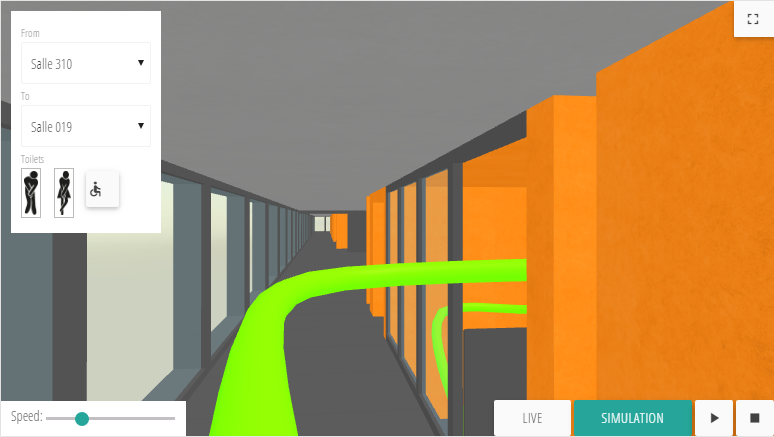
\includegraphics[width=0.9\linewidth]{ui-Spline}
	\caption{La courbe qui s'affiche à l'utilisateur.}
	\label{fig:ui-spline}
\end{figure}

Durant son parcours réel à l'intérieur du bâtiment, suivant le chemin trouvé par le système, il est important que l'utilisateur ait vraiment l'impression de se déplacer dans le bâtiment. La caméra effectue des mouvements qui sont linéaires et qui pourraient ressembler au déplacement d'un individu. La caméra projette le parcours quelques mètres devant elle afin que l'utilisateur puisse anticiper le chemin à parcourir.

\section{Localisation de l'utilisateur}
Un des objectifs fondamentaux de ce travail est de localiser l'utilisateur tout au long de son parcours. Cependant, après analyse (voir section \ref{sec:localisation}) des différentes technologies de le réaliser, nous nous sommes rendu compte que ce n'est malheureusement pas encore faisable. Chaque approche a présenté un ou plusieurs problèmes, résumés ci-dessous :
\begin{itemize}
	\item Le GPS ne fonctionne pas en intérieur;
	\item Les accès d'une page web sont insuffisants pour effectuer de la triangulation WiFi;
	\item Les navigateurs ne supportent pas encore l'API Bluetooth pour mettre en place une triangulation à l'aide de beacons bluetooth;
	\item Le niveau d'erreur de l'accéléromètre et du gyroscope est trop élevé, même pour faire une approximation de la position de l'utilisateur.
\end{itemize}

